\section*{Figure captions:}
\begin{figure}[H]
\begin{center}
\scalebox{0.85}{\includegraphics{fig1}}
\caption{
	a) shows the link between the components of the model.
	Solid lines mean the first component have a direct link on the second component.
	Dashed and double-headed lines represent a correlation or indirect link between the two components.
	b) visualizes the concavity ($b_3  = 1.25 > 1$) and convexity ($b_3 = 0.5 > 1$) of the power law relationship for allometric scaling of body size.
}
\label{fig1}
\end{center}
\end{figure}
%\vspace{-1.5cm} % E: consider \vfill
%\newpage
%
\begin{figure}[H]
\begin{center}
\scalebox{0.90}{\includegraphics{fig2}}
\caption{
	Different scenarios when net energy gain peaks at intermediate body size.
	The upper panels show the influence of resource availability.
	The lower panels show the influence of temperature when resources are unlimited.
	Low resource = 2.5 g, intermediate resource = 20 g, unlimited resource means an individual can collect 50 times its body mass, $b_2 = 0.75, a_2 = 20 a_1$, and $T_e = 15 ^{\circ} \rm{C}$.
	Low, intermediate, and high temperature = $5, 15, 25 ^{\circ} \rm{C}$.
	We assumed a high active metabolic rate $a_2 = 40 a_1, b_2  = 1.25$.
	Fixed parameter values: $b_1 = 0.75, \rho = 16$.
	Without warm-up.
}
\label{fig2}
\end{center}
\end{figure}
%\vspace{-1.5cm}
\newpage
%
\begin{figure}[H]
\begin{center}
\scalebox{0.85}{\includegraphics{fig3}}
\caption{
	 Daily net energy gain  $E_n$ as a function of body mass $z$ without warm-up, and foraging time limited to 0.5 hour.
	a) Daily net energy gain  $E_n$ as a function of body mass $z$ for different value of foraging exponent $b_3 = 0.5, 0.8, 1.25$, dashed, thin, thick lines respectively  at $T_e  = 15 ^{\circ} \rm{C}$.
	b) $E_n$ is maximized at an intermediate value of $z$  when shaded regions and resource quality $\rho$ intersect (i.e., \cref{eq:C1} is satisfied).
	Warm ($35^{\circ} \rm{C}$) and cold (15$^{\circ} \rm{C}$) environmental temperatures are denoted by red and cyan, respectively.
	The upper (lower) limit of the shaded region is $\widetilde{dE_n}$ ($\widetilde{E_n}$).
	c) Various shapes of $E_n$ based on b).
	In b) and c), $\rho = 13, 60, 100$ dashed, thin, and thick, respectively.
	Fixed parameter values: $b_1 = b_2 = 0.75, a_2 = 5 a_1, $.
}
\label{fig3}
\end{center}
\end{figure}
%\vspace{-1.5cm}
%\newpage
%
\begin{figure}[H]
\begin{center}
\scalebox{0.85}{\includegraphics{fig4}}
\caption{
	Lowest temperature required for the completion of warm-up as a function of body mass.
	a)  low value for conductance (0.1 $\times$ the default value).
	b) default value for conductance, wind speed  = 0.1m/s.
	c)  $a_w = 1.25$.
	Fixed parameter values: default conductance $K_1 = 0.05 \, c_p, r_3 = 0.5$.
	Remaining parameters are in \cref{table:table1}.
	The individual is given a maximum of 6 hours to complete warm-up.
	To focus on the effect of solar radiation, daily temperature is constant.
	Solar radiation increases linearly from 0 to 0.25 of the maximum value $S_0$ during a period of 6 hours.
}% Add parameter values later
\label{fig4}
\end{center}
\end{figure}
%\vspace{-1.5cm}
%\newpage
%
\begin{figure}[H]
\begin{center}
\scalebox{0.85}{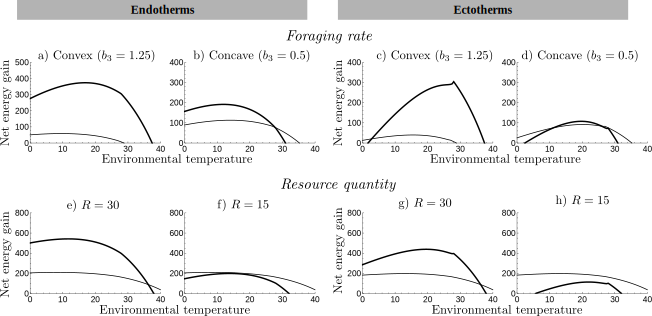
\includegraphics{fig5}}
\caption{
	Duration of warm-up as a function of the timing of warm-up.
	a) shows the effect of body size for ectotherms (the same thing for endotherm).
	b)  shows the effect of conductance for endotherms. Body size $z = 1$ , $a_w = 1.25$
	Solar radiation is equivalent to what would happen at 30 degree latitude during equinox.
	Daily temperature is fixed at $15^{\circ}\rm{C}$.
	Default value $K_1$ in a) and $K_2$ a) and b) .
}% Add parameter values later
\label{fig5}
\end{center}
\end{figure}
\vspace{-0.8cm}
%\newpage
%%
\begin{figure}%[H]
\begin{center}
\scalebox{0.85}{\includegraphics{fig6}}
\caption{
	Relationship between thermal performance and body size as function of other variables.
	a) when warm-up starts
	b) the exponent of foraging rate
	c) quantity of resource available.
	Parameters: ...
	 Net energy gain as a function of temperature.
	a) shows the effect of timing of warm-up ($\tau_f = 1$ hour and body size $z = 2$). %, early = sunrise, mid = sunrise+ 2 hr, late = sunrise + 4 hr
	b) shows the effect of the exponent $b_3$  for large $z= 2$ (thick) and small $z = 0.5$ (thin) body sizes, $\tau_f = 1$,.
	c) shows the effect of resource availability for large $z = 2$ (thick) and much smaller $z = 0.1$ (thin) body sizes.
	Solid (dashed) lines represent abundant (scarce) resource $R = 30, (15)$).
	Reduction in resource availability does not affect the much smaller individual so that solid and dashed lines overlap ($b_3 = b_2 = b_1 = 0.75$).
	Other parameters: $ b_2 = b_1  = 0.75,  a_2 = 10 a_1, a_w = 1.25$, and  $\rho = 30$.
}% Add non trivial units later
\label{fig6}
\end{center}
\end{figure}
